\documentclass[UTF-8]{article}
\usepackage{amsmath}
\usepackage{amssymb}
\usepackage{float}
\usepackage{graphicx}
\usepackage{epstopdf}
\usepackage{inputenc}
\usepackage{geometry}
\usepackage{pgfplots} 
\usepackage{listings}
\usepackage{enumitem}
\usepackage{lipsum}  
\usepackage{color}
\usepackage[colorlinks=true, urlcolor=blue, linkcolor=blue]{hyperref}
\geometry{left=2.5cm,right=2.5cm,top=2.5cm,bottom=2.5cm}

\definecolor{codegreen}{rgb}{0,0.6,0}
\definecolor{codegray}{rgb}{0.2,0.2,0.2}
\definecolor{codepurple}{rgb}{0.58,0,0.82}
\definecolor{backcolour}{rgb}{0.95,0.95,0.952}

\lstdefinestyle{mystyle}{
    backgroundcolor=\color{backcolour},   
    commentstyle=\color{codegreen},
    keywordstyle=\color{blue},
    numberstyle=\tiny\color{codegray},
    stringstyle=\color{codepurple},
    basicstyle=\ttfamily\footnotesize,
    breakatwhitespace=false,         
    breaklines=true,                 
    captionpos=b,                    
    keepspaces=true,                 
    numbers=left,                    
    numbersep=5pt,                  
    showspaces=false,                
    showstringspaces=false,
    showtabs=false,                  
    tabsize=2,
    linewidth=1.185\linewidth,
    resetmargins=true,
    xleftmargin=-1cm,
    xrightmargin=0.085\textwidth,
    prebreak = \raisebox{0ex}[0ex][0ex]{\ensuremath{\hookleftarrow}}
}

\lstset{style=mystyle}
\pgfplotsset{compat=1.18}

\title{High Performance Computing Proseminar 2024 \\
    \large Assignment 2} %exchange for assignment number

\author{Stefan Wagner \& Sebastian Bergner\\Team: Planning Desaster}
\begin{document}
    
    \maketitle
    
    \section*{Exercise 1}
    This exercise consists in writing a parallel application to speed up the computation of $\pi$.
    \\
    \\
    There are many ways of approximating $\pi$, one being a well-known Monte Carlo method: The ratio of the areas of a square and its incircle is $\pi/4$. Since the exact area of a circle cannot be computed (we don't know the value of $\pi$ yet), one can instead sample random points, check their distance from the center and compute the ratio of points inside the circle to all sampled points.
    
    \begin{itemize}
    	\item Write a sequential application `pi\_seq` in C or C++ that computes $\pi$ for a given number of samples (command line argument). Test your application for various, large sample sizes to verify the correctness of your implementation.
    	\\
     \\
    	The main part of the monte carlo pi approximation is shown below. The code works as follows: generate S random points inside a squared area, if they lie inside the unit circle the length of the vector they build is $\le 1$ thus we can increase the counter. Otherwise we just ignore it. In the end we have to multipy by 4 to accomodate the fact that we only generated random numbers in the right upper quadrant (no negative numbers).
    	\begin{lstlisting}[language=c]
double mc_pi(unsigned int S) {
	int in_count = 0;
	for(unsigned i = 0; i < S; ++i) {
		const double x = rand() / (double)RAND_MAX;
		const double y = rand() / (double)RAND_MAX;
		if(x * x + y * y <= 1.f) {
			in_count++;
		}
	}
	return 4.f * in_count / S;
}\end{lstlisting}
    	
    	
    	\item Consider a parallelization strategy using MPI. Which communication pattern(s) would you choose and why?
    	\\
     \\
    	As we actually don't have to accommodate relevant data that has to be distributed we can utilize the mpi reduce functionality. This should allow for least communication overhead. Each process gets its own share to work on the problem and initializes a random seed based on the rank it has. And after computing the elements inside the quarter circle we sum it up using reduce and then do the last step of the above function only in the master node (rank = 0).
    	
    	\item Implement your chosen parallelization strategy as a second application `pi\_mpi`. Run it with varying numbers of ranks and sample sizes and verify its correctness by comparing the output to `pi\_seq`.

In the below code section the main parts of the code are shown (boilerplate code has been omited).

\begin{lstlisting}[language=c]
int mc_pi(int S) {
    int in_count = 0;
    for(unsigned i = 0; i < S; ++i) {
        const double x = rand() / (double)RAND_MAX;
        const double y = rand() / (double)RAND_MAX;
        if(x * x + y * y <= 1.f) {
            in_count++;
        }
    }
    return in_count; // only return the number of elements inside
}

int main(int argc, char* argv[]) {
        // .. some boilerplate code left out
	MPI_Init(&argc, &argv); //start mpi
	// let every process work on their problem (we won't instruct them from the root node 0 only gather the data)
	int myRank, numProcesses;
	int insideLocal = 0;
	MPI_Comm_rank(MPI_COMM_WORLD, &myRank);
	MPI_Comm_size(MPI_COMM_WORLD, &numProcesses);

	srand(time(NULL)*myRank);

	int calculations_per_process = N/numProcesses;
	insideLocal = mc_pi(calculations_per_process);
	
	// here https://mpitutorial.com/tutorials/mpi-reduce-and-allreduce/ was quite helpful
	int insideGlobal = 0;
	MPI_Reduce(&insideLocal, &insideGlobal, 1, MPI_INT, MPI_SUM, 0, MPI_COMM_WORLD);

	if (myRank == 0){ // let only one rank do the last step
		double result = 4.f * insideGlobal / (N-(N%numProcesses)); // correction if N is not fully divisible by numProcesses
		// ... some more boilerplate code
	}
	MPI_Finalize();
	return 0;
}
\end{lstlisting}

     
     \begin{table}[H]
    \centering
        \begin{tabular}{|c|c|c|}
        \hline
        Problem size $10^N$ & serial result & parallel result \\ \hline 
        2 & 3.12          & 3.04            \\ \hline 
        3 & 3.132         & 3.032           \\ \hline 
        4 & 3.1712        & 3.1564          \\ \hline 
        5 & 3.141520      & 3.1392          \\ \hline 
        6 & 3.141664      & 3.143120        \\ \hline 
        7 & 3.141130      & 3.142680        \\ \hline 
        8 & 3.141698      & 3.141692        \\ \hline 
        9 & 3.141603      & 3.141559        \\\hline
        \end{tabular}
    \end{table}
    	
    	
            \begin{figure}
                \centering
                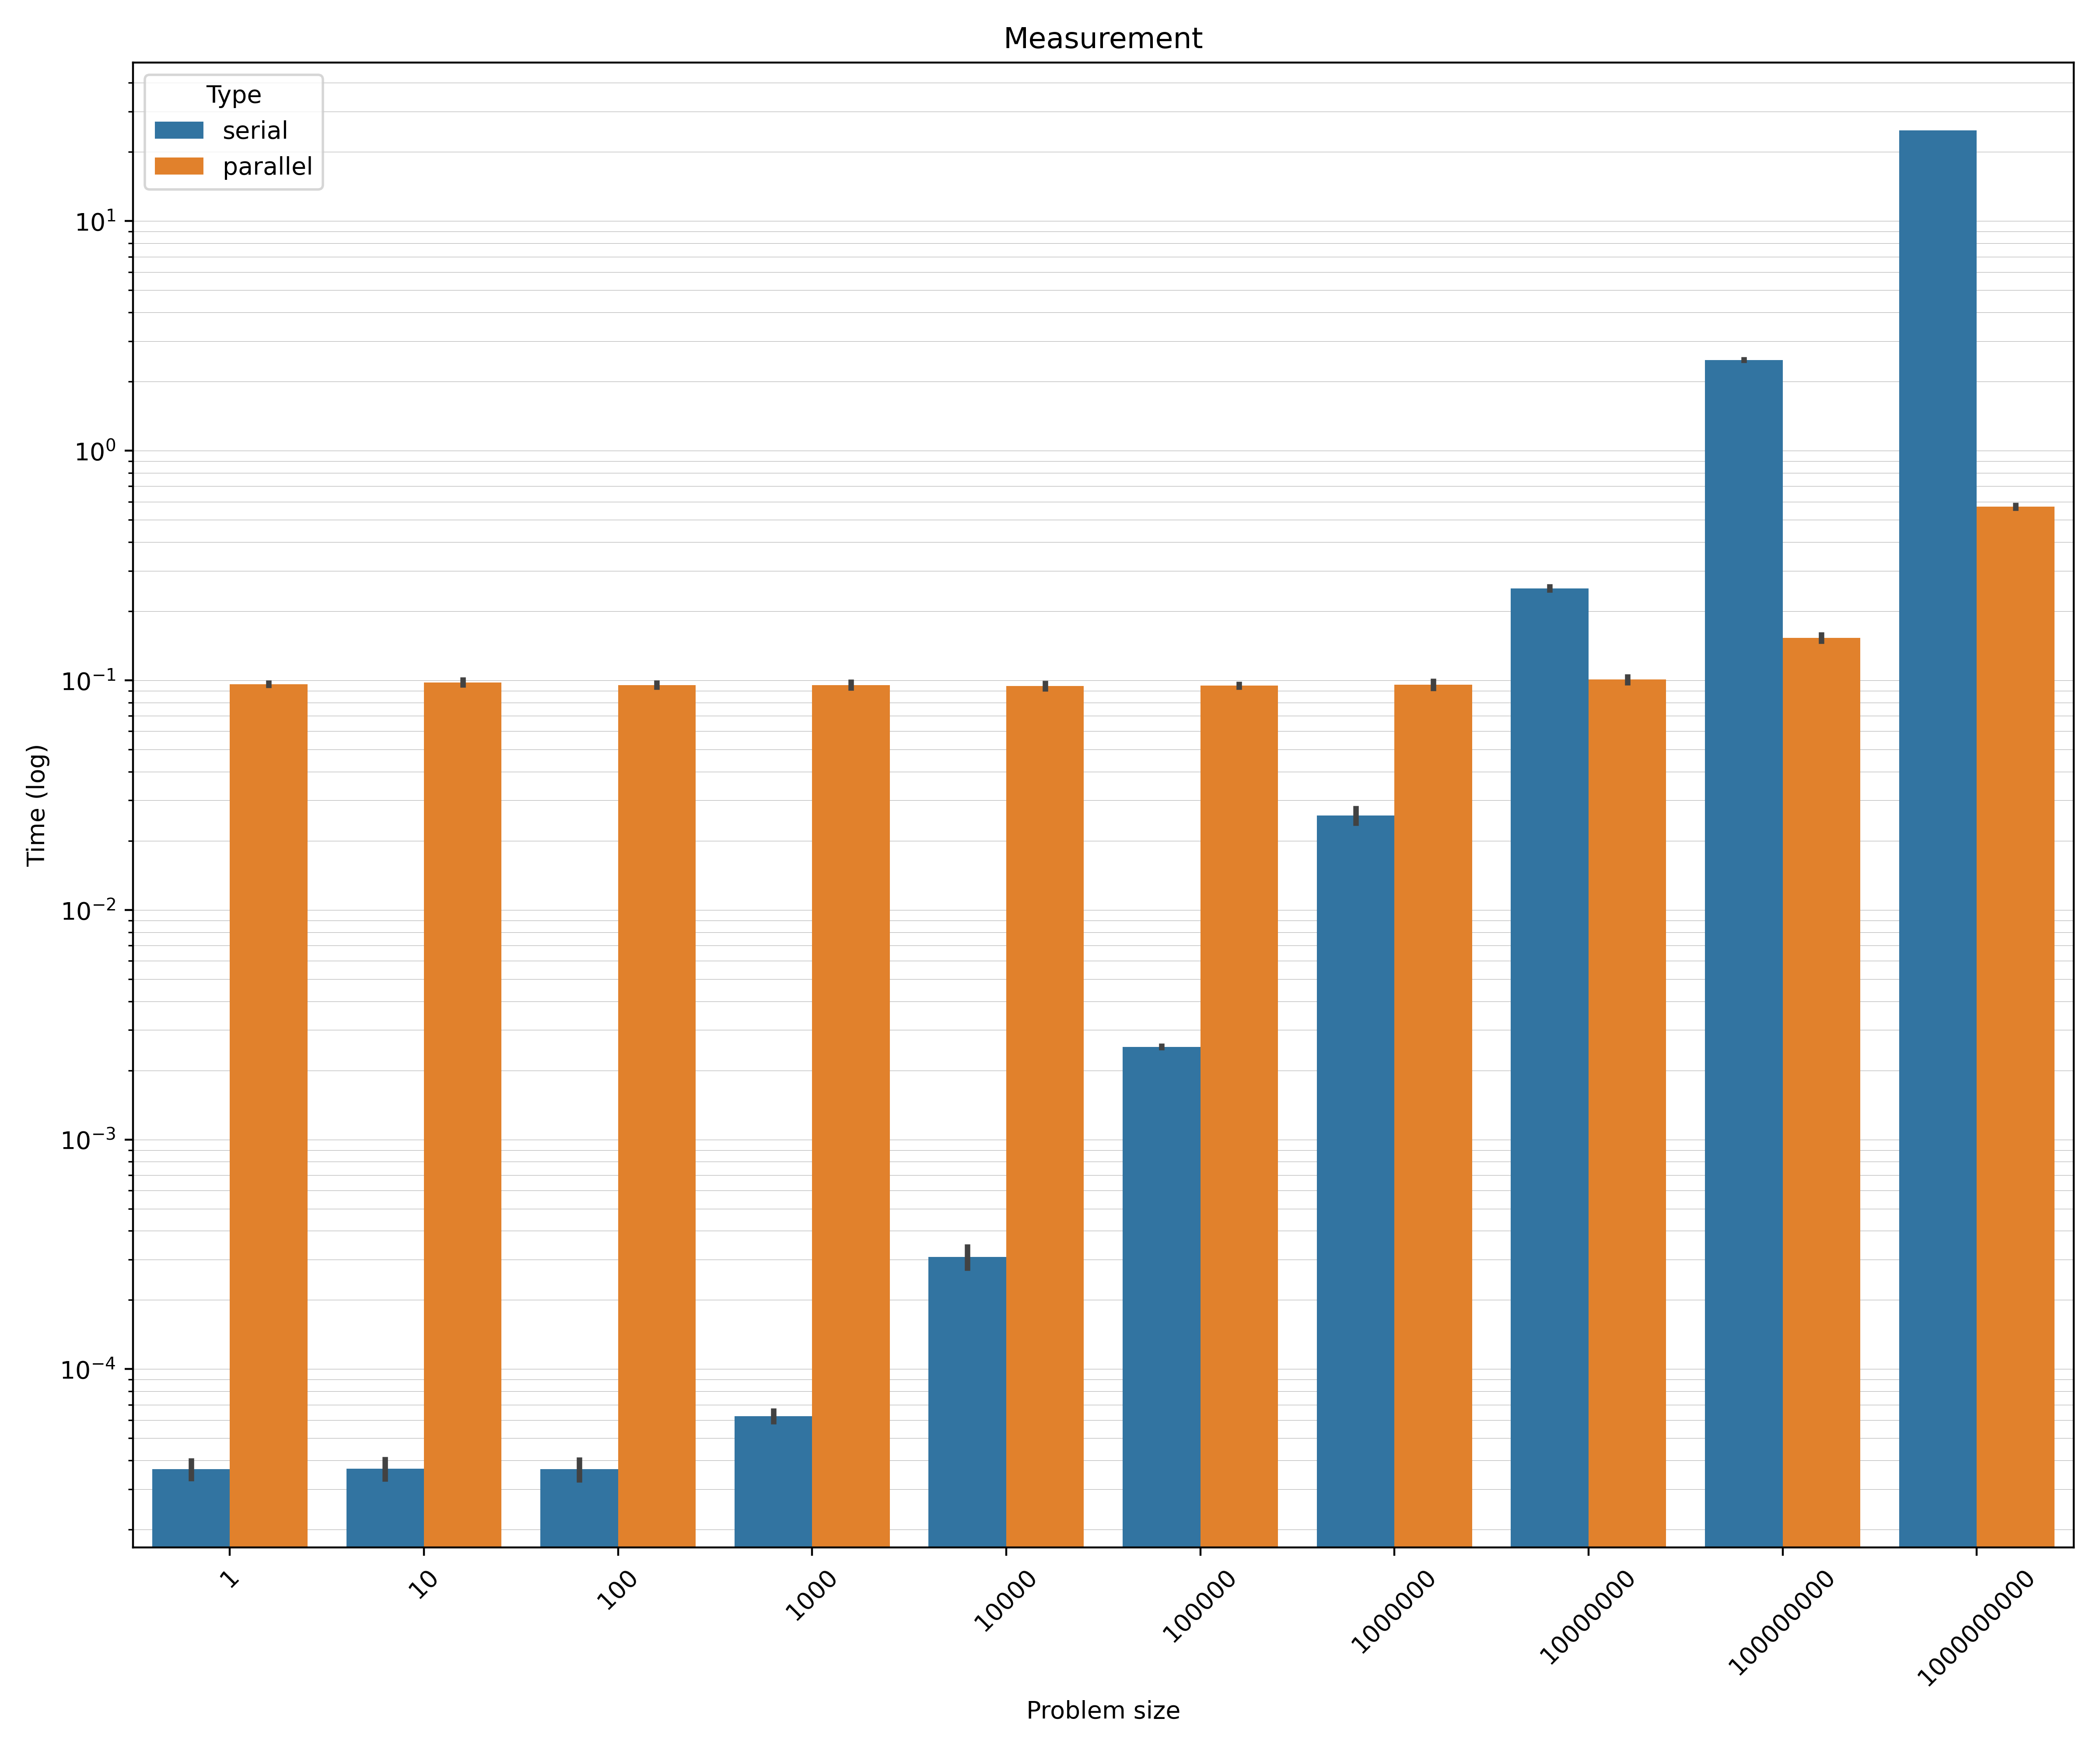
\includegraphics[width=0.75\linewidth]{figures/measurements_plot_mcpi.png}
                \caption{Monte Carlo Pi Approximation Measurements.}
                \label{fig:measurement_mcpi}
            \end{figure}
\begin{table}[]
\centering
    \begin{tabular}{|c|c|c|}
            
    	\hline
    	Problem size $10^N$ & Sequential Time [s] & Parallel Time [s] \\
    	\hline
    	2 & 0.0000366 & 0.0954576 \\
    	\hline
    	3 & 0.0000624 & 0.0954746 \\
    	\hline
    	4 & 0.0003084 & 0.0944174 \\
    	\hline
    	5 & 0.0025352 & 0.0947864 \\
    	\hline
    	6 & 0.0257526 & 0.0957872 \\
    	\hline
    	7 & 0.2516176 & 0.100753 \\
    	\hline
    	8 & 2.4850934 & 0.1531918 \\
    	\hline
    	9 & 24.8637024 & 0.5713218 \\
    	\hline
    \end{tabular}
\end{table}
\item Discuss the effects and implications of your parallelization. 
\\
\\
            This rather simple parallelization is able to offer an speedup of $\approx 43.6$ at the largest problem size we've measured. But looking at small problem sizes, the parallelized version has a rather high overhead of at least $\approx 95 ms$ (compared to an execution time of $41\mu s$ at 100 points). This can be seen in Fig. \ref{fig:measurement_mcpi}. So if we would want to have the best overall performing version we could find the limit where the parallel version performs better and switch between these two.
            
    	
    	\item Insert the measured wall time for $10^9$ samples for the sequential implementation and on 96 cores for MPI into the  \href{https://docs.google.com/spreadsheets/d/1p6d9F12EtykmI2-7MnHkg0U15UAtaCvWz8Ip92ZEsWo}{comparison spreadsheet}
    \end{itemize}
    
    
    \newpage
    \section*{Exercise 2}
	This exercise consists in parallelizing an application simulating the propagation of heat. A large class of scientific applications are so-called stencil applications. These simulate time-dependent physical processes such as the propagation of heat or pressure in a given medium. The core of the simulation operates on a grid and updates each cell with information from its neighbor cells.
	
	
	\begin{itemize}
		\item A sequential implementation of a 1-D heat stencil is available in heat\_stencil\_1D\_seq.c. Read the code and make sure you understand what happens. See the Wikipedia article on \href{https://en.wikipedia.org/wiki/Stencil_code}{Stencil Codes} for more information.
		\item Consider a parallelization strategy using MPI. Which communication pattern(s) would you choose and why? Are there additional changes required in the code beyond calling MPI functions? If so, elaborate!
            \begin{enumerate}[label*=\textbf{\alph *)}]
                \item \textbf{Complex Parallelization Strategy}\\
                First, we considered a rather complex communication pattern, as shown in Figure \ref{fig:parallelization_strategy_complex}.
                \begin{figure}[H]
                    \centering
                    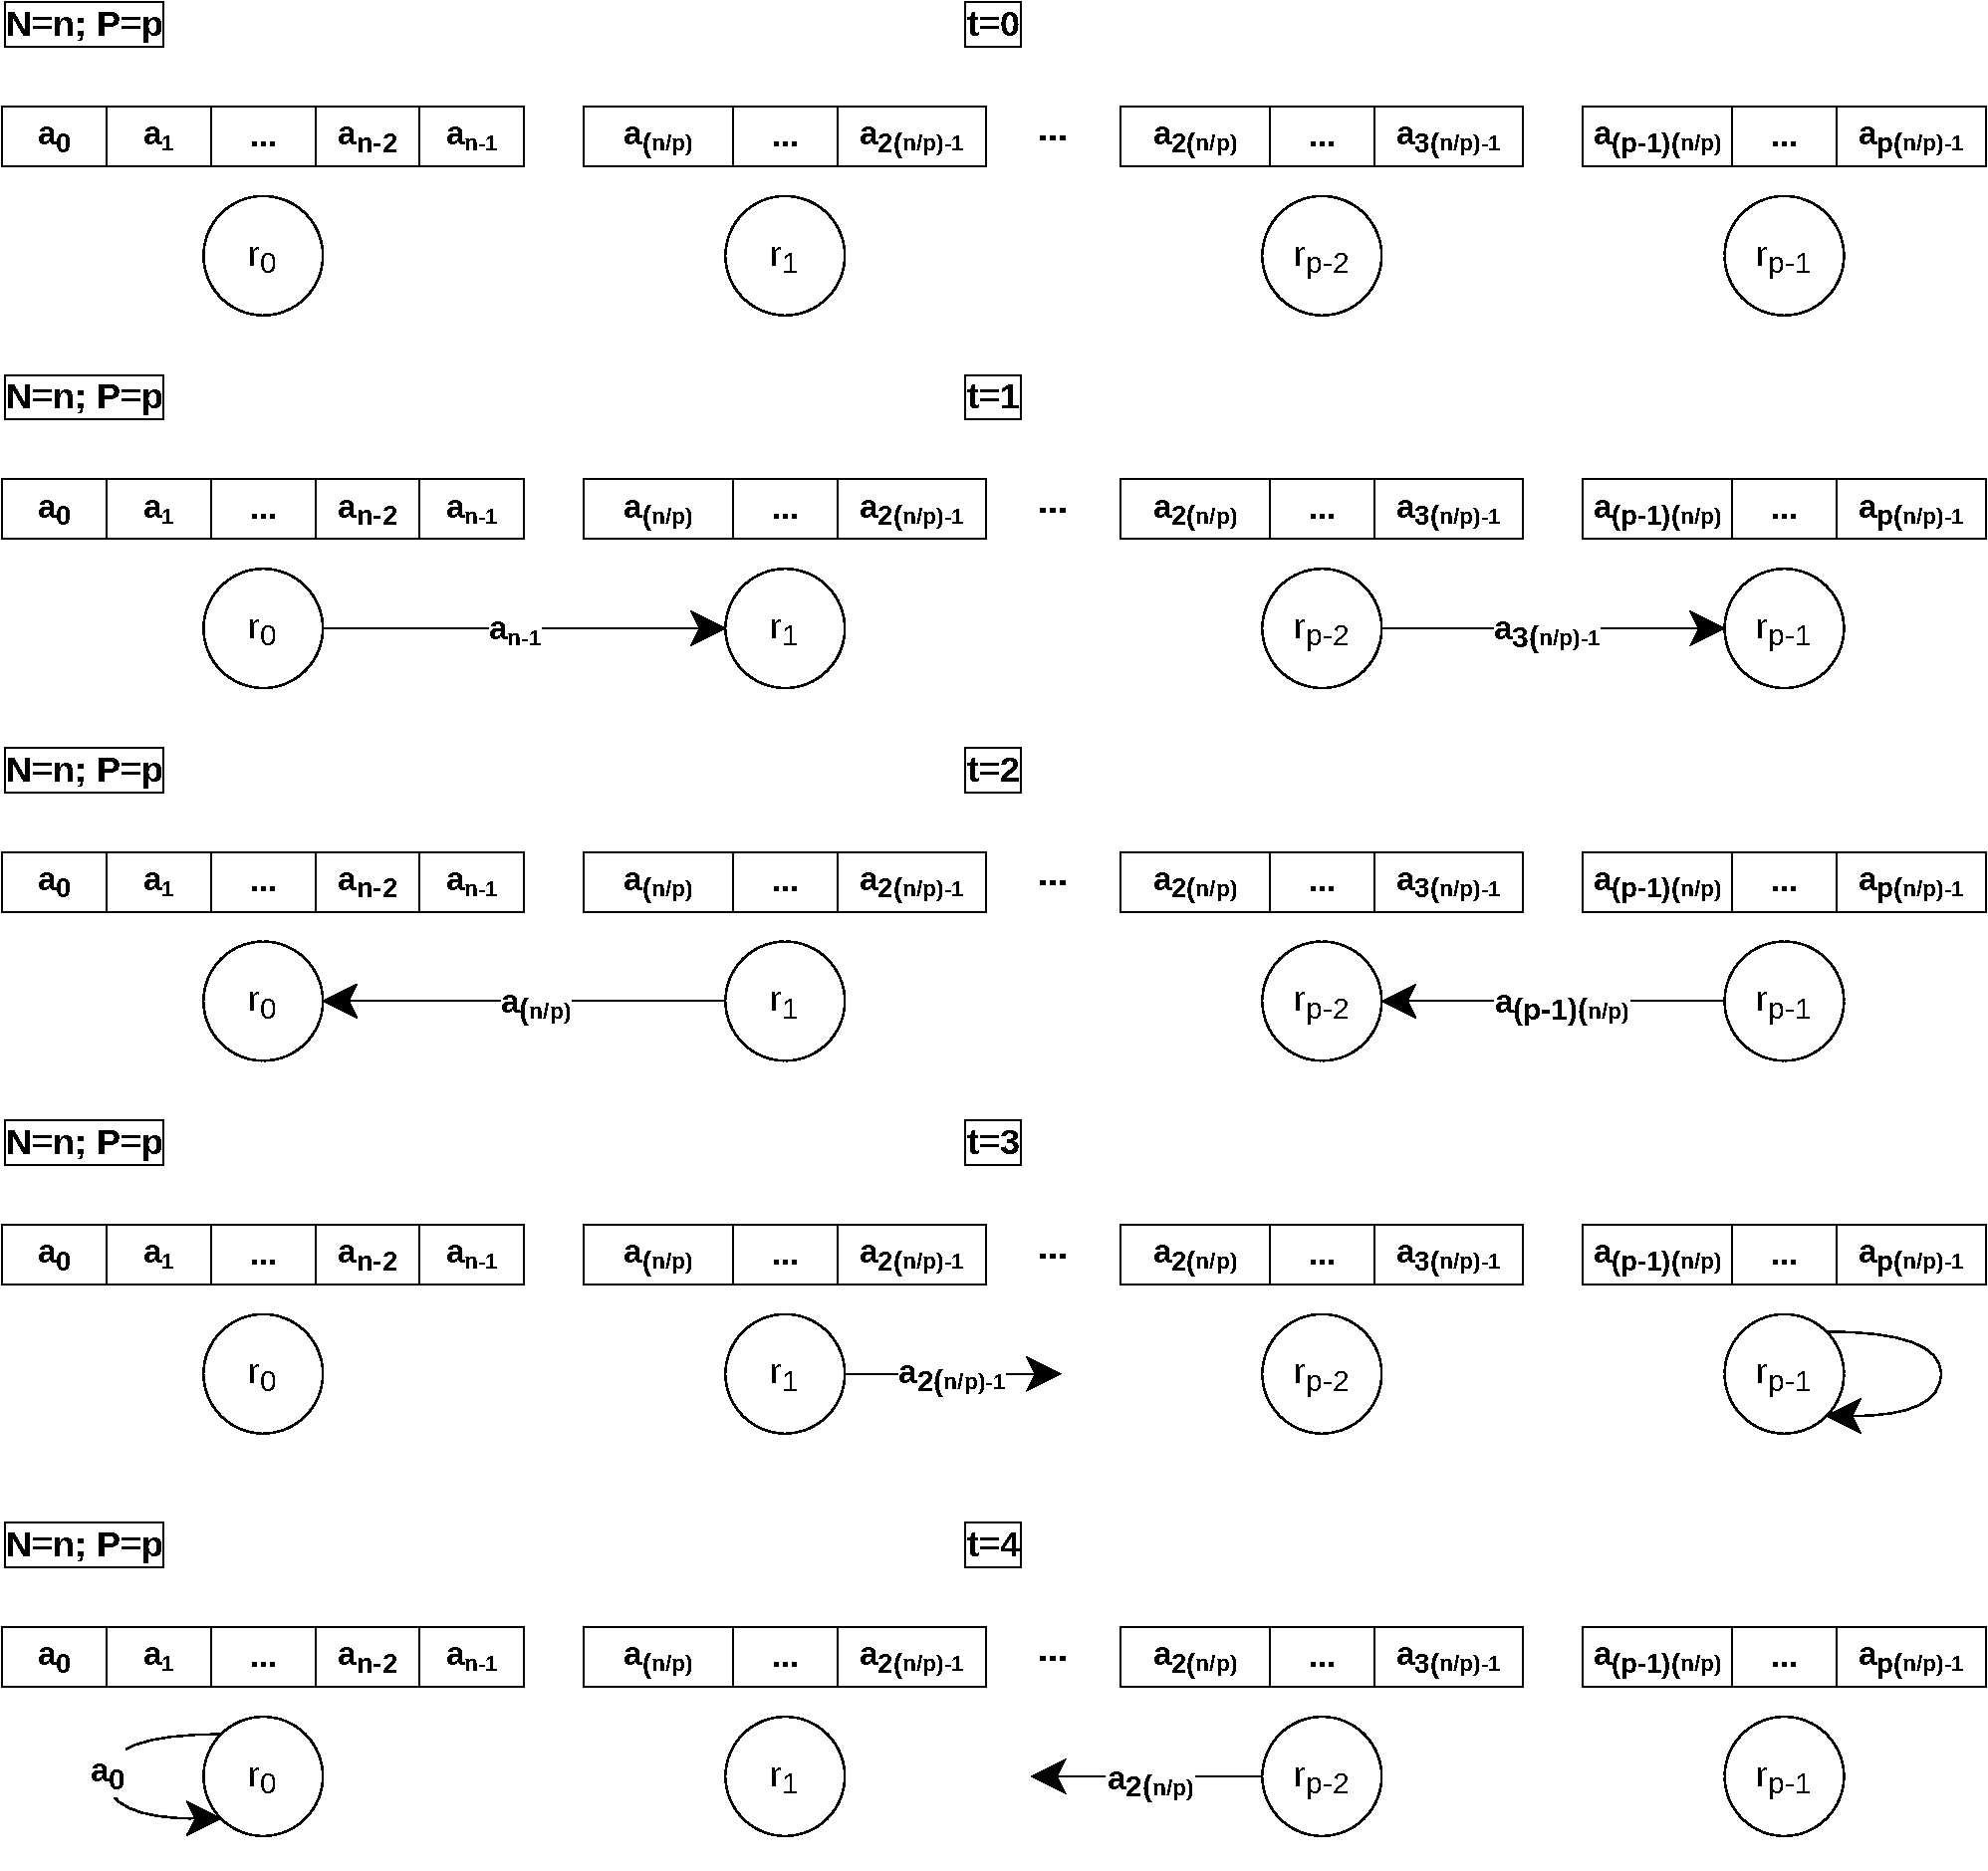
\includegraphics[width=1\linewidth]{figures/parallelization_strategy_complex.pdf}
                    \caption{Complex Parallelization Strategy}
                    \label{fig:parallelization_strategy_complex}
                \end{figure}
                The communication pattern is \textbf{blocking} and as follows:
                \begin{enumerate}[label=\textbf{\arabic *)}]
                    \item The total number of elements $N$ is distributed across $P$ vectors $V_p$, one vector per rank/process. Only rank $r_0$ holds a vector of length $N$ since it handles tasks like printing intermediate results. However, during computation, $r_0$ operates only on its own portion of the elements.
                    \item At $t=1$, all even-numbered ranks send their \textbf{last} element (except for $r_0$, where it is not the last) to their \textbf{right} neighbor, if one exists, while all odd-numbered ranks receive the element from their \textbf{left} neighbors.
                    \item At $t=2$, all odd-numbered ranks send their \textbf{first} element to their \textbf{left} neighbor, while all even-numbered ranks receive the element from their \textbf{right} neighbors, if one exists.
                    \item At $t=3$, all odd-numbered ranks send their \textbf{last} element to their \textbf{right} neighbor, while all even-numbered ranks receive the element from their \textbf{left} neighbors, if one exists.
                    \item At $t=4$, all even-numbered ranks send their \textbf{first} element to their \textbf{left} neighbor, while all odd-numbered ranks receive the element from their \textbf{right} neighbors, if one exists.
                    \item Now that all ranks have received the necessary information from their neighbors, they can begin their heat propagation computation.
                    \item If the \textbf{first} rank attempts to send to a non-existent \textbf{left} neighbor, or the \textbf{last} rank to a non-existent \textbf{right} neighbor, no element is sent. Instead, the receive buffer is populated with the first or last entry of vector $V$, respectively.
                    \item To print an intermediate or final result, all ranks send their portion of the elements to rank $r_0$, which holds a vector of size $N$, using \texttt{MPI\_Gather}. Rank $r_0$ then prints the complete result.\\
                \end{enumerate}
                \begin{itemize}
                    \item \textbf{Why did we choose this communication pattern?}\\
                    To parallelize the computation effectively, we need to distribute the problem size across all processes. However, due to the nature of the heat propagation calculation, each process requires the first and last elements from neighboring processes. To exchange this information while minimizing communication overhead (e.g. avoiding \texttt{MPI\_Scatter}), we focused solely on handling these edge cases.\\
                \end{itemize}
                \item \textbf{Simple Parallelization Strategy}\\
                After implementing the initial strategy and comparing the results with the data from the comparison spreadsheet, we decided to simplify the communication pattern, as illustrated in Figure \ref{fig:parallelization_strategy_simple}.\\\\
                The simpler communication pattern is now \textbf{non-blocking} and as follows:
                \begin{enumerate}[label=\textbf{\arabic *)}]
                    \item The total number of elements $N$ is distributed across $P$ vectors $V_p$, one vector per rank/process. Only rank $r_0$ holds a vector of length $N$ since it handles tasks like printing intermediate results. However, during computation, $r_0$ operates only on its own portion of the elements.
                    \item At $t=1$, \textbf{all} ranks first send their \textbf{first} and \textbf{last} elements (except for $r_0$, where it is not the last) to their \textbf{left} and \textbf{right} neighbors, if they exist, using the non-blocking \texttt{Isend()} call. Then, \textbf{all} ranks use the non-blocking \texttt{Irecv()} function to receive the \textbf{first} and \textbf{last} elements from their \textbf{right} and \textbf{left} neighbors, respectively.
                    \item At $t=2$, \textbf{all} ranks wait for the completion of their \texttt{Isend()} and \texttt{Irecv()} operations before starting the heat propagation computation.
                    \item If the \textbf{first} rank attempts to send to a non-existent \textbf{left} neighbor, or the \textbf{last} rank to a non-existent \textbf{right} neighbor, no element is sent. Instead, the receive buffer is populated with the first or last entry of vector $V$, respectively.
                    \item To print an intermediate or final result, all ranks send their portion of the elements to rank $r_0$, which holds a vector of size $N$, using \texttt{MPI\_Gather}. Rank $r_0$ then prints the complete result.\\
                \end{enumerate}
                \begin{figure}[H]
                    \centering
                    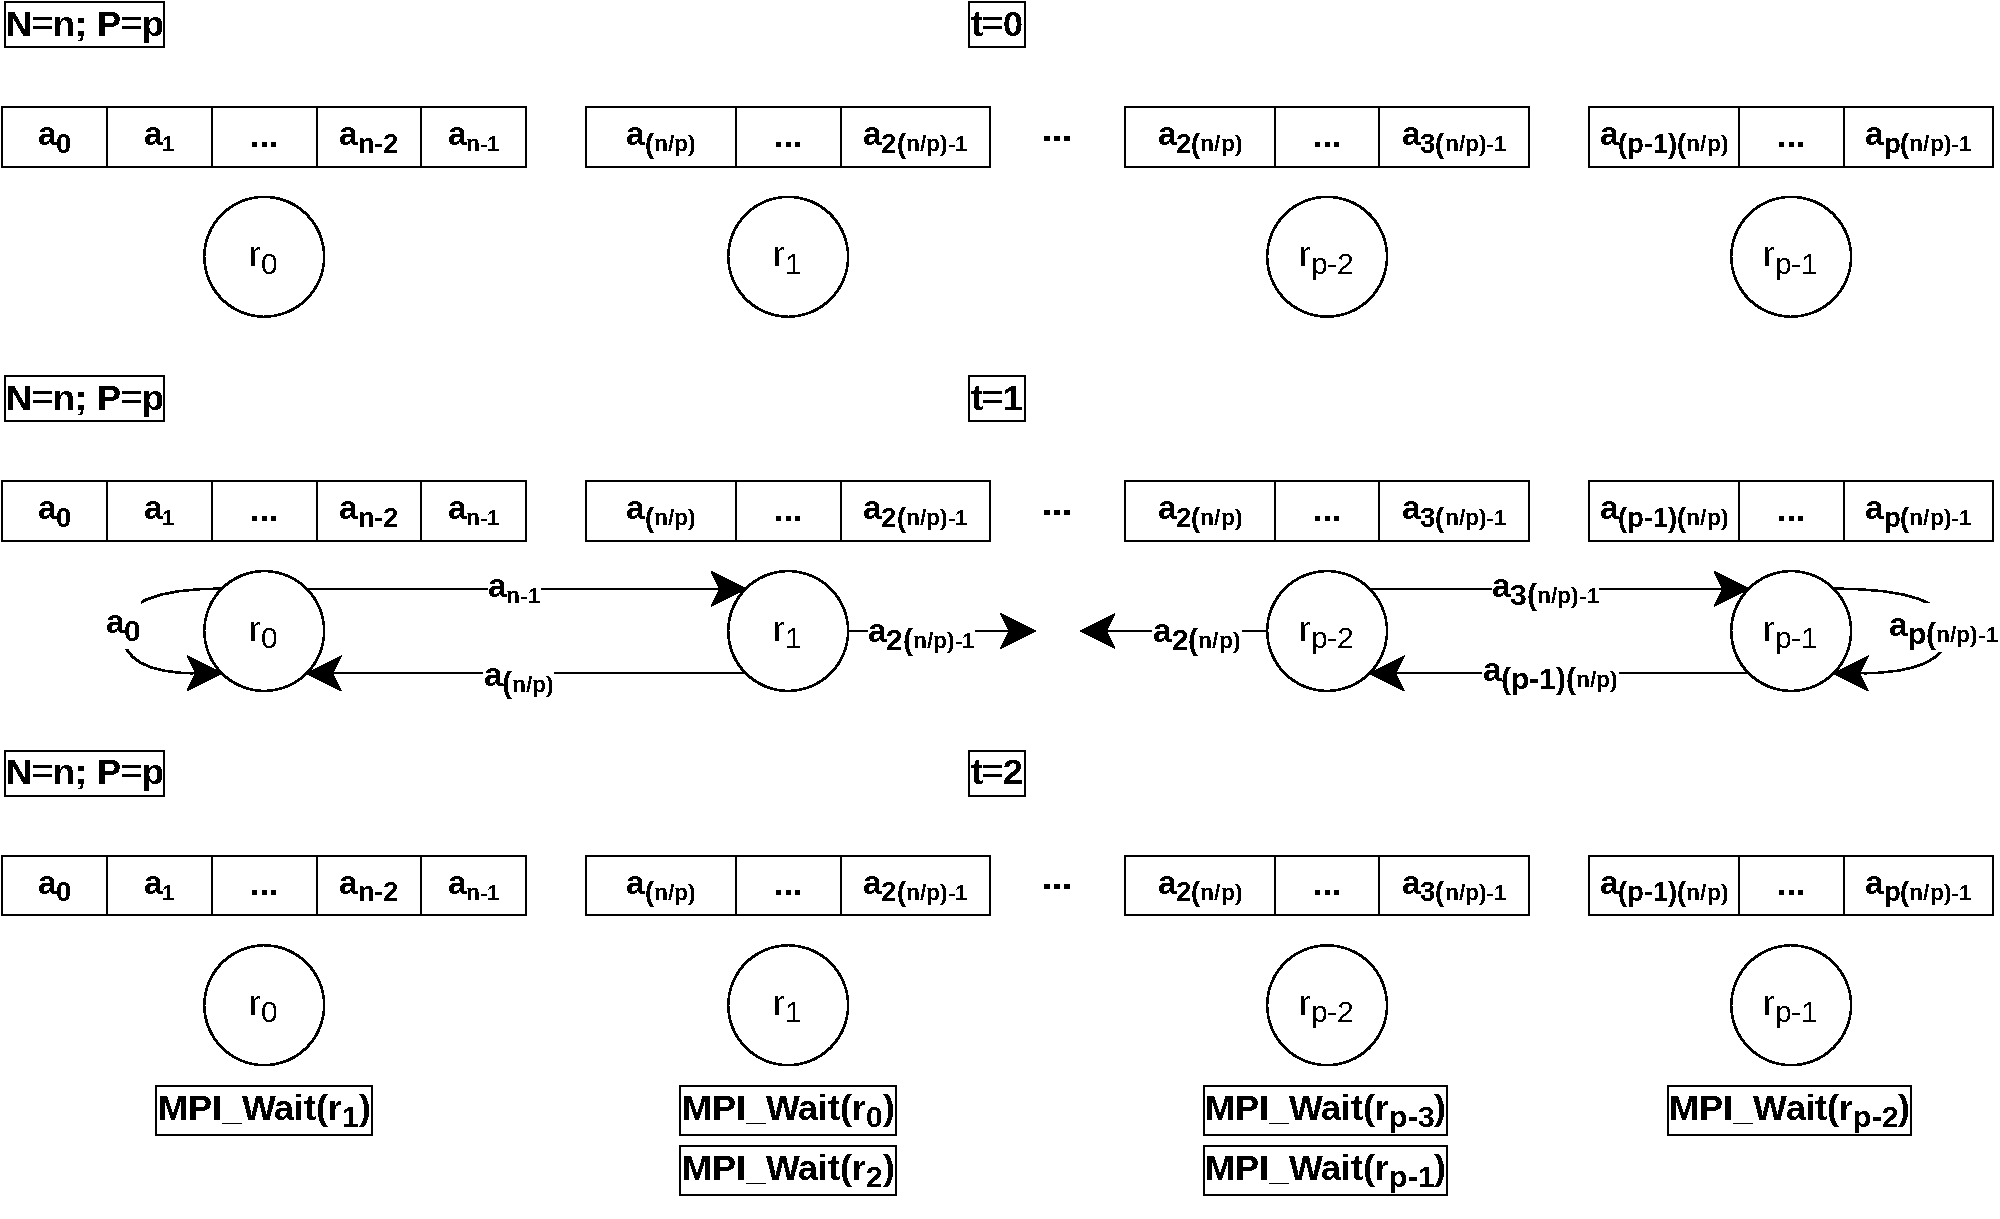
\includegraphics[width=1\linewidth]{figures/parallelization_strategy_simple.pdf}
                    \caption{Simple Parallelization Strategy}
                    \label{fig:parallelization_strategy_simple}
                \end{figure}
            \end{enumerate}
		\item Implement your chosen parallelization strategy as a second application `heat\_stencil\_1D\_mpi`. Run it with varying numbers of ranks and problem sizes and verify its correctness by comparing the output to `heat\_stencil\_1D\_seq`.
            \begin{enumerate}[label=\textbf{\arabic *)}]
                \item \textbf{heat\_stencil\_1D\_par\_complex.c}
% \resizebox{\textwidth}{!}{%
\begin{lstlisting}[language=c]
#include <stdio.h>
#include <stdlib.h>
#include <time.h>
#include <math.h>
#include <unistd.h>
#include <sys/stat.h>
#include <mpi.h>

typedef double value_t;
#define RESOLUTION 120

// -- vector utilities --
typedef value_t *Vector;
Vector createVector(int N);
void releaseVector(Vector m);
void printTemperature(Vector m, int N);

// -- measurment utilities --
#define FOLDER "output"
#define FILENAME "measurements.csv"
void timings_to_csv(unsigned problem_size, double time, int numRanks);

// -- simulation code ---
int main(int argc, char **argv) {
  clock_t start = clock();

  if(argc < 2){
		printf("Usage: %s <number of iterations>\n", argv[0]);
		return EXIT_FAILURE;
	}

  int N = atoi(argv[1]);
  int T = N * 500;

  MPI_Init(&argc, &argv);
  int myRank, numRanks;
  MPI_Comm_rank(MPI_COMM_WORLD, &myRank);
	MPI_Comm_size(MPI_COMM_WORLD, &numRanks);

  if (N % numRanks) {
    printf("Configuration not possible: N=%d, ranks=%d\n", N, numRanks);
    MPI_Finalize();
    return EXIT_FAILURE;
  }

  if (myRank == 0) {
    printf("Computing heat-distribution for room size N=%d for T=%d timesteps\n", N, T);
  }

  // ---------- setup ----------

  // create a buffer for storing temperature fields per rank
  int vector_size_per_rank = N / numRanks;
  Vector A = NULL;
  Vector B = NULL; // create a second buffer for the computation
  if (myRank == 0) {
    A = createVector(N);
    B = createVector(N);
  } else {
    A = createVector(vector_size_per_rank);
    B = createVector(vector_size_per_rank);
  }

  // set up initial conditions in A
  for (int i = 0; i < vector_size_per_rank; i++) {
    A[i] = 273; // temperature is 0 C everywhere (273 K)
  }

  // and there is a heat source somewhere
  int source_x = N / 4;
  int source_y = 273 + 60;

  int rank_with_source = source_x / vector_size_per_rank;
  if (myRank == 0) {
    A[source_x] = source_y;
  }
  if (myRank == rank_with_source) {
    A[source_x % vector_size_per_rank] = source_y;
  }

  if (myRank == 0) {
    printf("Initial:\t");
    printTemperature(A, N);
    printf("\n");
  }

  // ---------- compute ----------
  value_t t_from_previous_rank = 0;
  value_t t_from_next_rank = 0;

  // for each time step ..
  for (int t = 0; t < T; t++) {
    // communication between ranks to get temperatures of adjacent cells
    if (myRank % 2 == 0) {
      if (myRank != numRanks-1) {
        // send last temperature to next rank
        MPI_Send(&A[vector_size_per_rank-1], 1, MPI_DOUBLE, myRank+1, 0, MPI_COMM_WORLD);
        // receive first temperature from next rank
        MPI_Recv(&t_from_next_rank, 1, MPI_DOUBLE, myRank+1, 0, MPI_COMM_WORLD, MPI_STATUS_IGNORE);
      } else {
        t_from_next_rank = A[vector_size_per_rank-1];
      }

      if (myRank != 0) {
        // receive last temperature from previous rank
        MPI_Recv(&t_from_previous_rank, 1, MPI_DOUBLE, myRank-1, 0, MPI_COMM_WORLD, MPI_STATUS_IGNORE);
        // send first temperature to previous rank
        MPI_Send(&A[0], 1, MPI_DOUBLE, myRank-1, 0, MPI_COMM_WORLD);
      } else {
        t_from_previous_rank = A[0];
      }
    } else {
      // receive last temperature from previous rank
      MPI_Recv(&t_from_previous_rank, 1, MPI_DOUBLE, myRank-1, 0, MPI_COMM_WORLD, MPI_STATUS_IGNORE);
      // send first temperature to previous rank
      MPI_Send(&A[0], 1, MPI_DOUBLE, myRank-1, 0, MPI_COMM_WORLD);

      if (myRank != numRanks-1) {
        // send last temperature to next rank
        MPI_Send(&A[vector_size_per_rank-1], 1, MPI_DOUBLE, myRank+1, 0, MPI_COMM_WORLD);
        // receive first temperature from next rank
        MPI_Recv(&t_from_next_rank, 1, MPI_DOUBLE, myRank+1, 0, MPI_COMM_WORLD, MPI_STATUS_IGNORE);
      } else {
        t_from_next_rank = A[vector_size_per_rank-1];
      }
    }

    // .. we propagate the temperature
    for (long long i = 0; i < vector_size_per_rank; i++) {
      // center stays constant (the heat is still on)
      if (myRank == rank_with_source && i == (source_x % vector_size_per_rank)) {
        B[i] = A[i];
        continue;
      }

      // get temperature at current position
      value_t tc = A[i];

      // get temperatures of adjacent cells
      value_t tl = (i != 0) ? A[i - 1] : t_from_previous_rank;
      value_t tr = (i != vector_size_per_rank - 1) ? A[i + 1] : t_from_next_rank;

      // compute new temperature at current position
      B[i] = tc + 0.2 * (tl + tr + (-2 * tc));
    }

    // swap matrices (just pointers, not content)
    Vector H = A;
    A = B;
    B = H;

    // show intermediate step
    if (!(t % 10000)) {
      // Gather all data from all ranks to rank 0
      MPI_Gather(A, vector_size_per_rank, MPI_DOUBLE, A, vector_size_per_rank, MPI_DOUBLE, 0, MPI_COMM_WORLD);
      if (myRank == 0) {
        printf("Step t=%d:\t", t);
        printTemperature(A, N);
        printf("\n");
      }
    }
  }
  
  releaseVector(B);

  MPI_Gather(A, vector_size_per_rank, MPI_DOUBLE, A, vector_size_per_rank, MPI_DOUBLE, 0, MPI_COMM_WORLD);
  int success = 1;

  if (myRank == 0) {
    // measure time
    clock_t end = clock();
    double total_time = ((double)(end - start)) / CLOCKS_PER_SEC;
    timings_to_csv(N, total_time, numRanks);

    // ---------- check ----------
    printf("Final:\t\t");
    printTemperature(A, N);
    printf("\n");

    int success = 1;
    for (long long i = 0; i < N; i++) {
      value_t temp = A[i];
      if (273 <= temp && temp <= 273 + 60)
        continue;
      success = 0;
      break;
    }

    printf("Verification: %s\n", (success) ? "OK" : "FAILED");
    printf("Wall Clock Time = %f seconds\n", total_time);
  }

  // ---------- cleanup ----------
  releaseVector(A);
  MPI_Finalize();

  // done
  return (success) ? EXIT_SUCCESS : EXIT_FAILURE;
}

Vector createVector(int N) {
  // create data and index vector
  return malloc(sizeof(value_t) * N);
}

void releaseVector(Vector m) { free(m); }

void printTemperature(Vector m, int N) {
  const char *colors = " .-:=+*^X#%@";
  const int numColors = 12;

  // boundaries for temperature (for simplicity hard-coded)
  const value_t max = 273 + 60;
  const value_t min = 273 + 0;

  // set the 'render' resolution
  int W = RESOLUTION;

  // step size in each dimension
  int sW = N / W;

  // room
  // left wall
  printf("X");
  // actual room
  for (int i = 0; i < W; i++) {
    // get max temperature in this tile
    value_t max_t = 0;
    for (int x = sW * i; x < sW * i + sW; x++) {
      max_t = (max_t < m[x]) ? m[x] : max_t;
    }
    value_t temp = max_t;

    // pick the 'color'
    int c = ((temp - min) / (max - min)) * numColors;
    c = (c >= numColors) ? numColors - 1 : ((c < 0) ? 0 : c);

    // print the average temperature
    printf("%c", colors[c]);
  }
  // right wall
  printf("X");
}

void timings_to_csv(unsigned problem_size, double time, int numRanks) {
	FILE* fpt;
	int set_header = 0;
  char full_filepath[1024];
  sprintf(full_filepath, "%s/%s", FOLDER, FILENAME);
  if(access(FOLDER, F_OK) != 0) mkdir(FOLDER, 0755);
	if(access(full_filepath, F_OK) != 0) set_header = 1;
	fpt = fopen(full_filepath, "a+");
	if(set_header) fprintf(fpt, "Impl/Ranks,Problem Size,Time\n");
	fprintf(fpt, "par_complex/%d,%u,%.9f\n", numRanks, problem_size, time);
	fclose(fpt);
}
\end{lstlisting}
% }
                \item \textbf{heat\_stencil\_1D\_par\_simple.c}
\begin{lstlisting}[language=c]
int main(int argc, char **argv) {
  clock_t start = clock();

  if(argc < 2){
		printf("Usage: %s <number of iterations>\n", argv[0]);
		return EXIT_FAILURE;
	}

  int N = atoi(argv[1]);
  int T = N * 500;

  MPI_Init(&argc, &argv);
  int myRank, numRanks;
  MPI_Comm_rank(MPI_COMM_WORLD, &myRank);
	MPI_Comm_size(MPI_COMM_WORLD, &numRanks);

  if (N % numRanks) {
    if (myRank == 0) {
      printf("Configuration not possible: N=%d, ranks=%d\n", N, numRanks);
    }
    MPI_Finalize();
    return EXIT_FAILURE;
  }
  if (myRank == 0) {
    printf("Computing heat-distribution for room size N=%d for T=%d timesteps\n", N, T);
  }

  // ---------- setup ----------

  // create a buffer for storing temperature fields per rank
  int vector_size_per_rank = N / numRanks;
  Vector A = NULL;
  Vector B = NULL;
  if (myRank == 0) {
    A = createVector(N);
    B = createVector(N);
  } else {
    A = createVector(vector_size_per_rank);
    B = createVector(vector_size_per_rank);
  }

  // set up initial conditions in A
  for (int i = 0; i < vector_size_per_rank; i++) {
    A[i] = 273; // temperature is 0 C everywhere (273 K)
  }

  // and there is a heat source somewhere
  int source_x = N / 4;
  int source_y = 273 + 60;

  int rank_with_source = source_x / vector_size_per_rank;
  if (myRank == 0) {
    A[source_x] = source_y;
  }
  if (myRank == rank_with_source) {
    A[source_x % vector_size_per_rank] = source_y;
  }

  if (myRank == 0) {
    printf("Initial:\t");
    printTemperature(A, N);
    printf("\n");
  }
  MPI_Request requests[4];
  // ---------- compute ----------

  // for each time step ..
  for (int t = 0; t < T; t++) {
    // sync with other ranks
    value_t t_left, t_right;
    if (myRank != 0 && myRank != numRanks-1){ //consider edge cases separatelly
      MPI_Isend(&A[vector_size_per_rank-1], 1, MPI_DOUBLE, myRank+1, 0, MPI_COMM_WORLD, &requests[0]);
      MPI_Isend(&A[0], 1, MPI_DOUBLE, myRank-1, 0, MPI_COMM_WORLD, &requests[1]);

      MPI_Irecv(&t_left, 1, MPI_DOUBLE, myRank-1, 0, MPI_COMM_WORLD, &requests[2]);
      MPI_Irecv(&t_right, 1, MPI_DOUBLE, myRank+1, 0, MPI_COMM_WORLD, &requests[3]);
      
      MPI_Wait(&requests[2], MPI_STATUS_IGNORE);
      MPI_Wait(&requests[3], MPI_STATUS_IGNORE);
    }
    else if(myRank == 0){ // edge case 1 first rank
      MPI_Isend(&A[vector_size_per_rank-1], 1, MPI_DOUBLE, myRank+1, 0, MPI_COMM_WORLD, &requests[0]);
      MPI_Irecv(&t_right, 1, MPI_DOUBLE, myRank+1, 0, MPI_COMM_WORLD, &requests[1]);
      t_left = A[0];
    }
    else{ // edge case 1 last rank
      MPI_Isend(&A[0], 1, MPI_DOUBLE, myRank-1, 0, MPI_COMM_WORLD, &requests[0]);
      MPI_Irecv(&t_left, 1, MPI_DOUBLE, myRank-1, 0, MPI_COMM_WORLD, &requests[1]);
      t_right = A[vector_size_per_rank-1];
    }
    // pre-calc syncing done
    MPI_Wait(&requests[0], MPI_STATUS_IGNORE);
    MPI_Wait(&requests[1], MPI_STATUS_IGNORE);


    // .. we propagate the temperature
    for (long long i = 0; i < vector_size_per_rank; i++) {
      // center stays constant (the heat is still on)
      if (myRank == rank_with_source && i == (source_x%vector_size_per_rank)) {
        B[i] = A[i];
        continue;
      }

      // get temperature at current position
      value_t tc = A[i];

      // get temperatures of adjacent cells
      value_t tl = (i != 0) ? A[i - 1] : t_left;
      value_t tr = (i != vector_size_per_rank - 1) ? A[i + 1] : t_right;

      // compute new temperature at current position
      B[i] = tc + 0.2 * (tl + tr + (-2 * tc));
    }

    // swap matrices (just pointers, not content)
    Vector H = A;
    A = B;
    B = H;

    // show intermediate step
    if (!(t % 10000)) {
      // now we have to gather all data in rank 0
      MPI_Gather(A, vector_size_per_rank, MPI_DOUBLE, A, vector_size_per_rank, MPI_DOUBLE, 0, MPI_COMM_WORLD);

      if (myRank == 0){
        printf("Step t=%d:\t", t);
        printTemperature(A, N);
        printf("\n");
      }
    }
  }

  releaseVector(B);
  int success = 1;
  // last sync
  MPI_Gather(A, vector_size_per_rank, MPI_DOUBLE, A, vector_size_per_rank, MPI_DOUBLE, 0, MPI_COMM_WORLD);
  if (myRank == 0){
    // measure time
    clock_t end = clock();
    double total_time = ((double)(end - start)) / CLOCKS_PER_SEC;
    timings_to_csv(N, total_time, numRanks);

    // ---------- check ----------

    printf("Final:\t\t");
    printTemperature(A, N);
    printf("\n");

    
    for (long long i = 0; i < N; i++) {
      value_t temp = A[i];
      if (273 <= temp && temp <= 273 + 60)
        continue;
      success = 0;
      break;
    }

    printf("Verification: %s\n", (success) ? "OK" : "FAILED");
    printf("Wall Clock Time = %f seconds\n", total_time);
  }

  // ---------- cleanup ----------

  releaseVector(A);

  MPI_Finalize();
  // done
  return (success) ? EXIT_SUCCESS : EXIT_FAILURE;
\end{lstlisting}
            \end{enumerate}
            \pagebreak
		\item Discuss the effects and implications of your parallelization.
            \begin{table}[H]
            \centering
            \begin{tabular}{|lllllllll|}
            \hline
            \multicolumn{9}{|c|}{\textbf{Results of 1D Heat Stencil Execution (5 Repetitions)}} \\ \hline
            \multicolumn{1}{|c|}{\textbf{Impl/Ranks}} &
              \multicolumn{8}{c|}{\textbf{Problem Size}} \\ \hline
            \multicolumn{1}{|c|}{\textbf{}} &
              \multicolumn{2}{c|}{768} &
              \multicolumn{2}{c|}{1536} &
              \multicolumn{2}{c|}{3072} &
              \multicolumn{2}{c|}{6144} \\ \hline
            \multicolumn{1}{|l|}{} &
              \multicolumn{1}{l|}{$\mu$} &
              \multicolumn{1}{l|}{$\sigma$} &
              \multicolumn{1}{l|}{$\mu$} &
              \multicolumn{1}{l|}{$\sigma$} &
              \multicolumn{1}{l|}{$\mu$} &
              \multicolumn{1}{l|}{$\sigma$} &
              \multicolumn{1}{l|}{$\mu$} &
              $\sigma$ \\ \hline
            \multicolumn{1}{|l|}{seq/1} &
              \multicolumn{1}{l|}{0.56} &
              \multicolumn{1}{l|}{0.0} &
              \multicolumn{1}{l|}{2.38} &
              \multicolumn{1}{l|}{0.01} &
              \multicolumn{1}{l|}{9.65} &
              \multicolumn{1}{l|}{0.02} &
              \multicolumn{1}{l|}{38.47} &
              0.1 \\ \hline
            \multicolumn{1}{|l|}{par\_complex/2} &
              \multicolumn{1}{l|}{0.8} &
              \multicolumn{1}{l|}{0.0} &
              \multicolumn{1}{l|}{2.82} &
              \multicolumn{1}{l|}{0.02} &
              \multicolumn{1}{l|}{10.83} &
              \multicolumn{1}{l|}{0.29} &
              \multicolumn{1}{l|}{42.78} &
              2.08 \\ \hline
            \multicolumn{1}{|l|}{par\_simple/2} &
              \multicolumn{1}{l|}{0.75} &
              \multicolumn{1}{l|}{0.0} &
              \multicolumn{1}{l|}{2.74} &
              \multicolumn{1}{l|}{0.01} &
              \multicolumn{1}{l|}{10.79} &
              \multicolumn{1}{l|}{0.49} &
              \multicolumn{1}{l|}{41.47} &
              0.05 \\ \hline
            \multicolumn{1}{|l|}{par\_complex/6} &
              \multicolumn{1}{l|}{0.66} &
              \multicolumn{1}{l|}{0.0} &
              \multicolumn{1}{l|}{1.75} &
              \multicolumn{1}{l|}{0.04} &
              \multicolumn{1}{l|}{5.17} &
              \multicolumn{1}{l|}{0.02} &
              \multicolumn{1}{l|}{17.28} &
              0.03 \\ \hline
            \multicolumn{1}{|l|}{par\_simple/6} &
              \multicolumn{1}{l|}{0.53} &
              \multicolumn{1}{l|}{0.0} &
              \multicolumn{1}{l|}{1.46} &
              \multicolumn{1}{l|}{0.01} &
              \multicolumn{1}{l|}{4.62} &
              \multicolumn{1}{l|}{0.01} &
              \multicolumn{1}{l|}{16.19} &
              0.04 \\ \hline
            \multicolumn{1}{|l|}{par\_complex/12} &
              \multicolumn{1}{l|}{0.58} &
              \multicolumn{1}{l|}{0.03} &
              \multicolumn{1}{l|}{1.32} &
              \multicolumn{1}{l|}{0.01} &
              \multicolumn{1}{l|}{3.46} &
              \multicolumn{1}{l|}{0.01} &
              \multicolumn{1}{l|}{10.38} &
              0.02 \\ \hline
            \multicolumn{1}{|l|}{par\_simple/12} &
              \multicolumn{1}{l|}{\textbf{0.44}} &
              \multicolumn{1}{l|}{0.01} &
              \multicolumn{1}{l|}{\textbf{1.07}} &
              \multicolumn{1}{l|}{0.01} &
              \multicolumn{1}{l|}{\textbf{2.95}} &
              \multicolumn{1}{l|}{0.03} &
              \multicolumn{1}{l|}{9.34} &
              0.05 \\ \hline
            \multicolumn{1}{|l|}{par\_complex/24} &
              \multicolumn{1}{l|}{1.48} &
              \multicolumn{1}{l|}{0.01} &
              \multicolumn{1}{l|}{2.93} &
              \multicolumn{1}{l|}{0.02} &
              \multicolumn{1}{l|}{6.02} &
              \multicolumn{1}{l|}{0.02} &
              \multicolumn{1}{l|}{12.82} &
              0.04 \\ \hline
            \multicolumn{1}{|l|}{par\_simple/24} &
              \multicolumn{1}{l|}{0.82} &
              \multicolumn{1}{l|}{0.01} &
              \multicolumn{1}{l|}{1.61} &
              \multicolumn{1}{l|}{0.01} &
              \multicolumn{1}{l|}{3.44} &
              \multicolumn{1}{l|}{0.02} &
              \multicolumn{1}{l|}{7.64} &
              0.03 \\ \hline
            \multicolumn{1}{|l|}{par\_complex/48} &
              \multicolumn{1}{l|}{1.49} &
              \multicolumn{1}{l|}{0.0} &
              \multicolumn{1}{l|}{2.93} &
              \multicolumn{1}{l|}{0.02} &
              \multicolumn{1}{l|}{5.86} &
              \multicolumn{1}{l|}{0.03} &
              \multicolumn{1}{l|}{12.18} &
              0.02 \\ \hline
            \multicolumn{1}{|l|}{par\_simple/48} &
              \multicolumn{1}{l|}{0.85} &
              \multicolumn{1}{l|}{0.01} &
              \multicolumn{1}{l|}{1.63} &
              \multicolumn{1}{l|}{0.01} &
              \multicolumn{1}{l|}{3.31} &
              \multicolumn{1}{l|}{0.02} &
              \multicolumn{1}{l|}{7.22} &
              0.05 \\ \hline
            \multicolumn{1}{|l|}{par\_complex/96} &
              \multicolumn{1}{l|}{1.55} &
              \multicolumn{1}{l|}{0.02} &
              \multicolumn{1}{l|}{2.98} &
              \multicolumn{1}{l|}{0.01} &
              \multicolumn{1}{l|}{5.94} &
              \multicolumn{1}{l|}{0.03} &
              \multicolumn{1}{l|}{11.93} &
              0.08 \\ \hline
            \multicolumn{1}{|l|}{par\_simple/96} &
              \multicolumn{1}{l|}{0.83} &
              \multicolumn{1}{l|}{0.01} &
              \multicolumn{1}{l|}{1.6} &
              \multicolumn{1}{l|}{0.03} &
              \multicolumn{1}{l|}{3.14} &
              \multicolumn{1}{l|}{0.02} &
              \multicolumn{1}{l|}{\textbf{6.5}} &
              0.02 \\ \hline
            \end{tabular}
            \caption{1D Stencil Measurements}
            \label{table:measurement_1dstencil}
            \end{table}
            \begin{figure}[H]
                \centering
                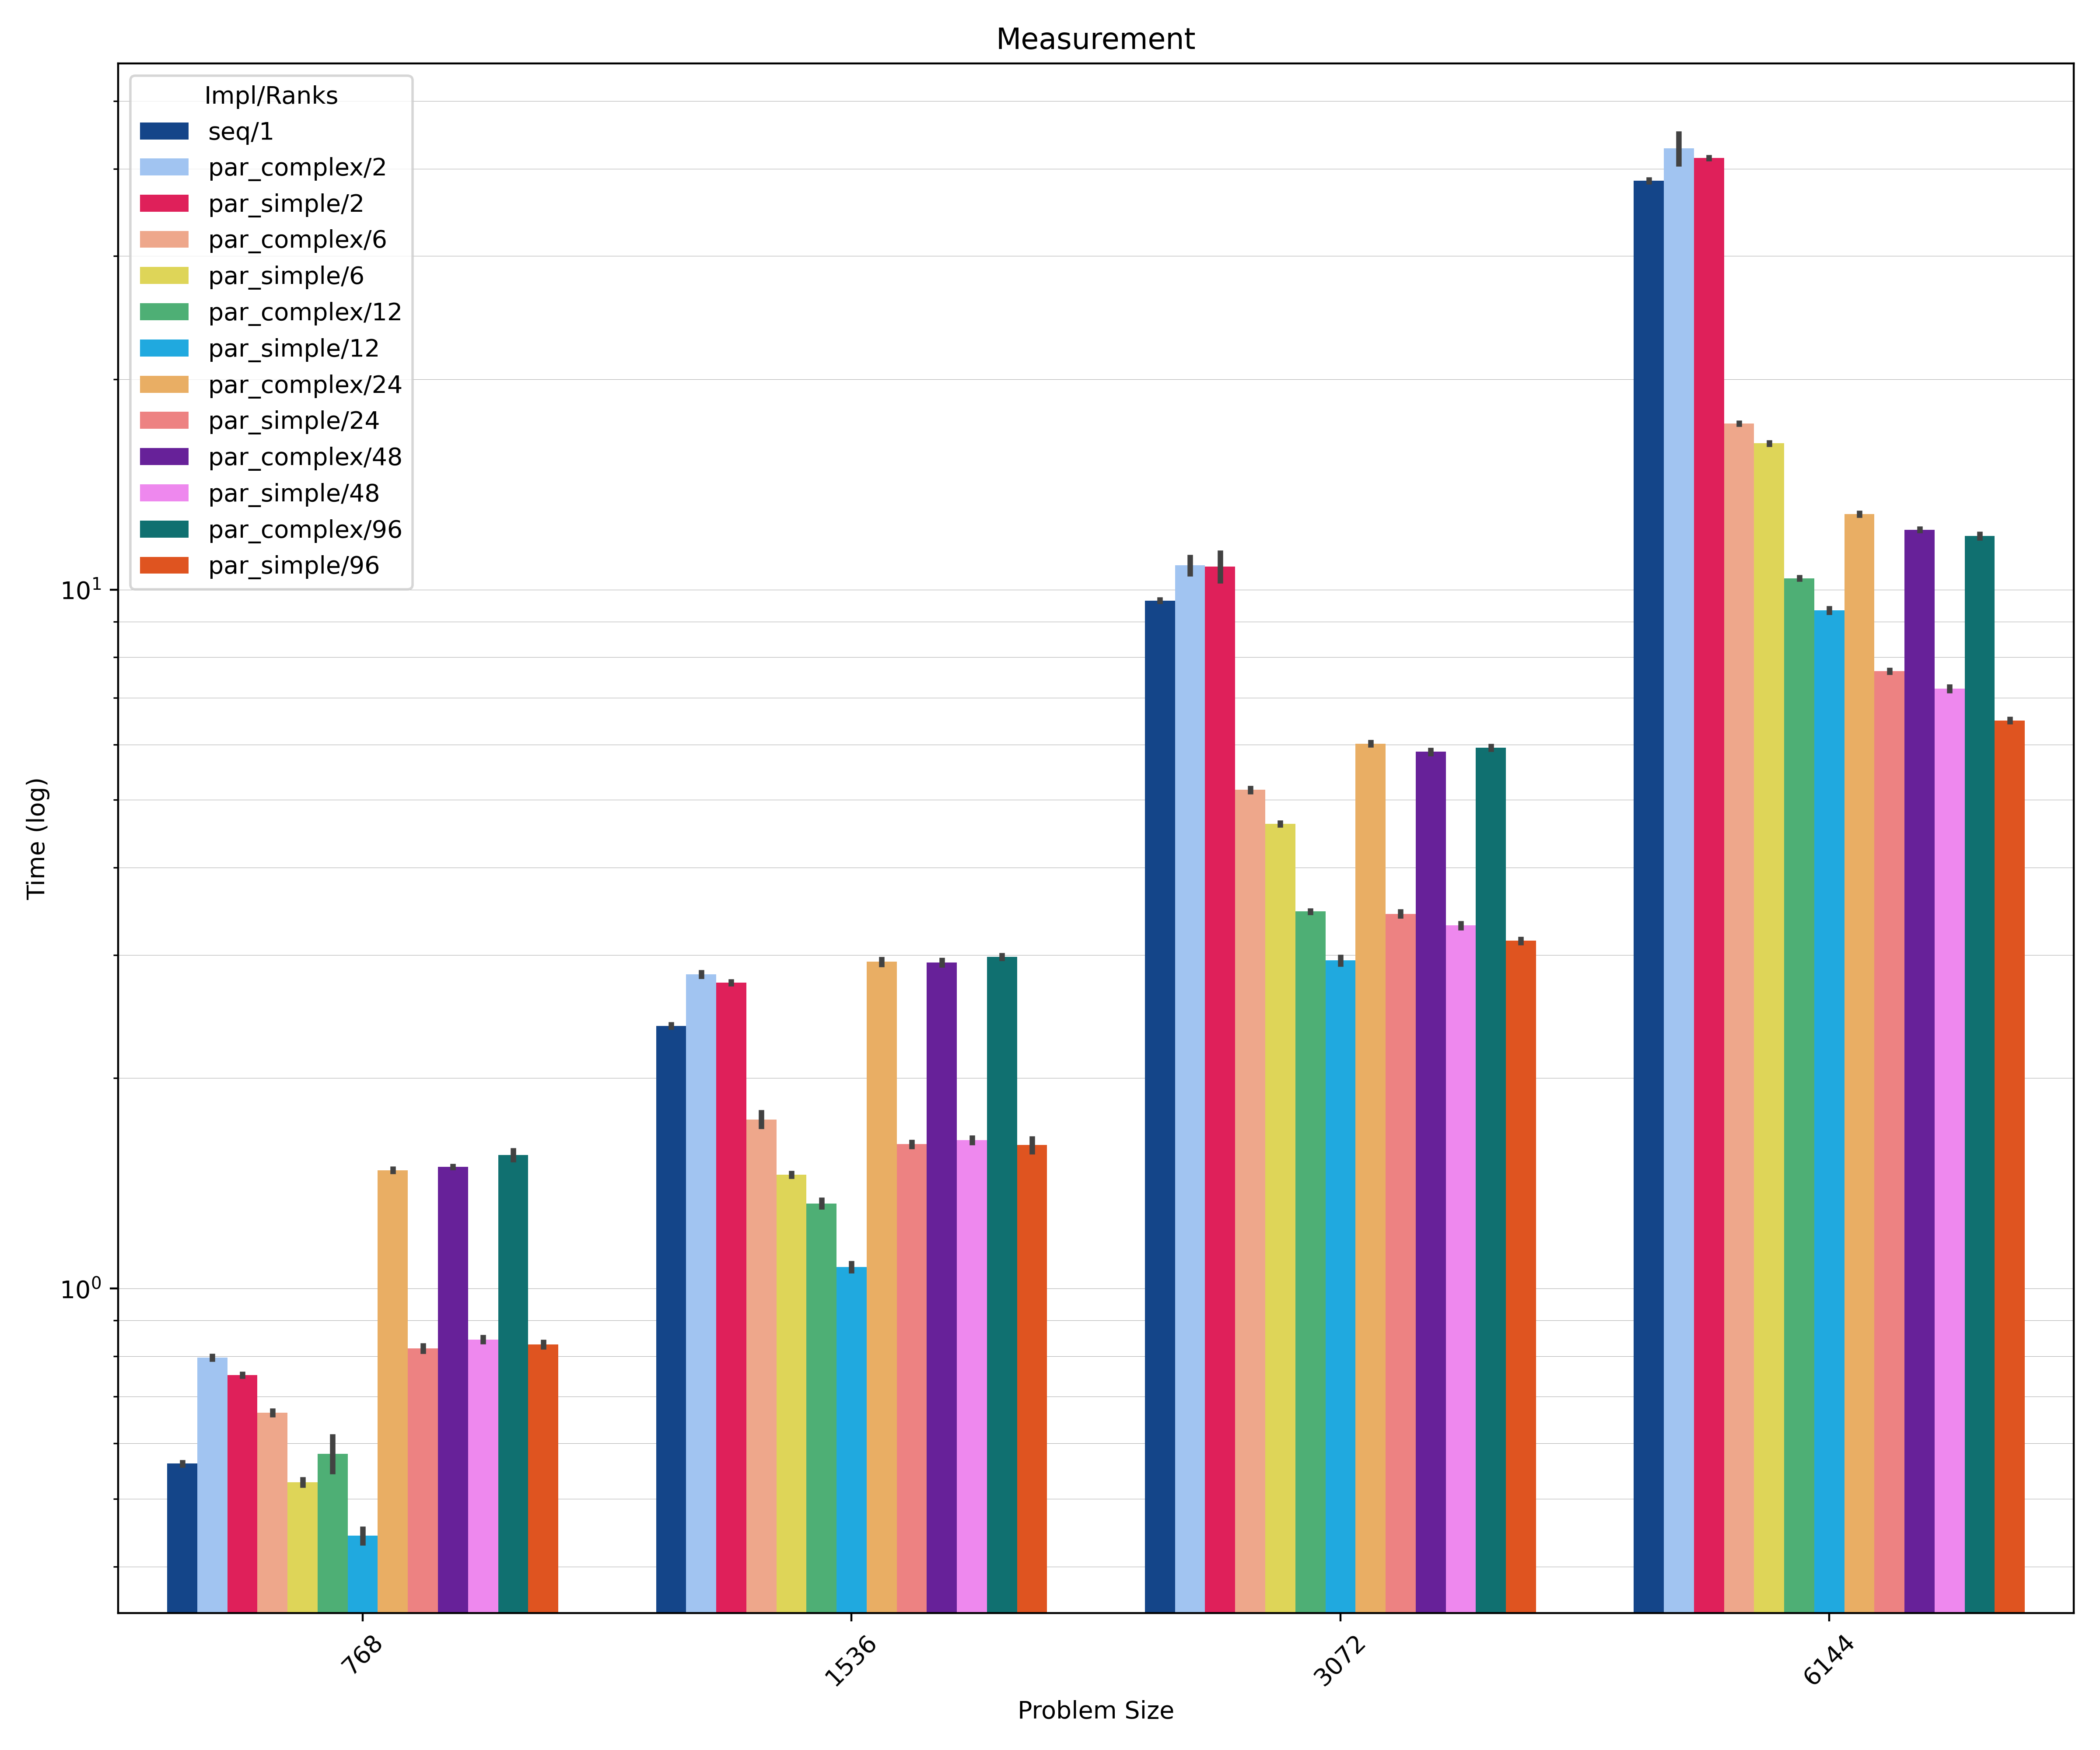
\includegraphics[width=0.9\linewidth]{figures/measurements_plot_1Dstencil.png}
                \caption{1D Stencil Measurements.}
                \label{fig:measurement_1dstencil}
            \end{figure}
            The measurements of the 1D stencil heat propagation algorithms, as discussed earlier, are displayed in Table \ref{table:measurement_1dstencil} and illustrated in Figure \ref{fig:measurement_1dstencil}.\\
            \begin{itemize}
                \item \textbf{Sequential vs. Parallel Execution}:\\
                The sequential version \texttt{seq/1} has the longest execution times, especially at larger problem sizes (e.g. 6144). The parallel implementations \texttt{par\_complex} and \texttt{par\_simple} significantly reduce execution time compared to the sequential version across all problem sizes. This shows that parallelization improves performance as the number of ranks increases.
                \item \textbf{Performance at Different Ranks}:\\
                The execution time decreases with an increase in the number of ranks for both the \texttt{par\_complex} and \texttt{par\_simple} versions. This suggests that the workload is being effectively distributed across more resources. For higher ranks, especially between 48 and 96, performance gains diminish, with little difference in execution time.
                \item \textbf{Complex vs. Simple Implementations}:\\
                The \texttt{par\_simple} version consistently outperforms \texttt{par\_complex} due to its use of non-blocking MPI calls, which allow ranks to continue processing while communication occurs. This approach is faster because MPI efficiently manages the communication order, ensuring all ranks receive the correct information with minimal delays. In contrast, the \texttt{par\_complex} version uses a blocking communication pattern, where ranks must wait to send and receive messages sequentially, leading to slower performance.
                \item \textbf{Standard Deviation and Stability}:
                The standard deviation $\sigma$ values are very low across all implementations and ranks, which suggests that the measurements are stable and there is little variation between repetitions. 
            \end{itemize}
		\item Insert the measured wall time for N=6144 and 96 cores into the  \href{https://docs.google.com/spreadsheets/d/1p6d9F12EtykmI2-7MnHkg0U15UAtaCvWz8Ip92ZEsWo}{comparison spreadsheet}
	\end{itemize}


\end{document}